\section{General Reasoning}
\label{sec:reasoning}

%An explanation of how the data and models come together to inform your core hypothesis or hypotheses.

\begin{figure*}
	\centering
		\subfloat[{\small BERT}]{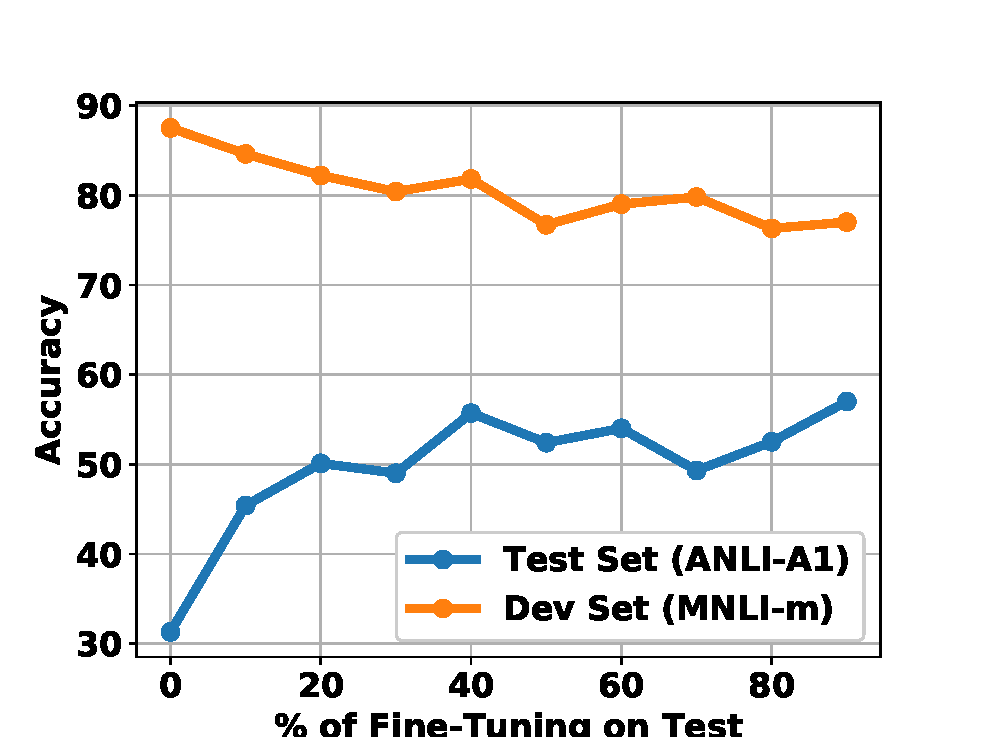
\includegraphics[width=0.45\textwidth]{Figs4Paper/percentage_finetuned_vs_accuracy_roberta.eps}}
		\subfloat[{\small RoBERTa}]{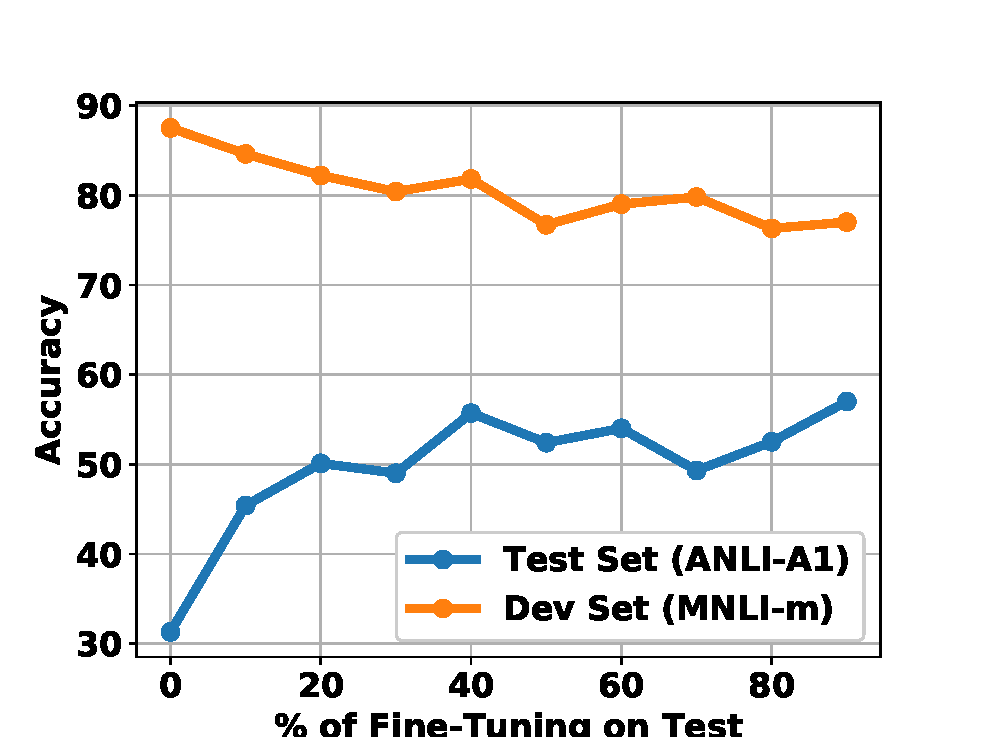
\includegraphics[width=0.45\textwidth]{Figs4Paper/percentage_finetuned_vs_accuracy_roberta.eps}}
	\caption{Inoculation by fine-tuning on the test set}
	\label{fig:inoculation}
\end{figure*}

Our hypothesis is that that the failings in NLI adversarial evaluation come from the use of singular datasets used to develop the model. To avoid this we introduce a wide range of datasets as part of our train set.  On the model side, we have two state-of-the art models: BERT\textsubscript{BASE} and RoBERTa\textsubscript{BASE} which perform exceedingly well in standard NLI tasks. By diversifying our training data, we aim to show that these two models can also do well in the NLI adversarial evaluation setting.